\section{Interfejs Użytkownika. Zofia Sosińska}\label{chap:ui}

Projekt Interfejsu Użytkownika przewiduje trzy trybu: zwykły, budowania oraz walki. Zadaniem każdego z nich będzie odzwierciedlenie aktualnej wiedzy granej postaci. Gracz musi widzieć proste podsumowanie wszystkich najważniejszych informacji.
	Tryb zwykły przewiduje podstawowe funkcje, takie jak pokazanie:
surowców i funduszy,
aktualnego czasu w grze, 
kompasu pokazującego także wrogów i ważnych lokacji,
ikon postaci, na które gracz może się przełączyć;
Inspiracją dla górnego paska z informacjami oraz dla ikon dostępnych postaci jest ten użyty w grze Warcraft 3.

\begin{figure}[htbp]
    \centering
    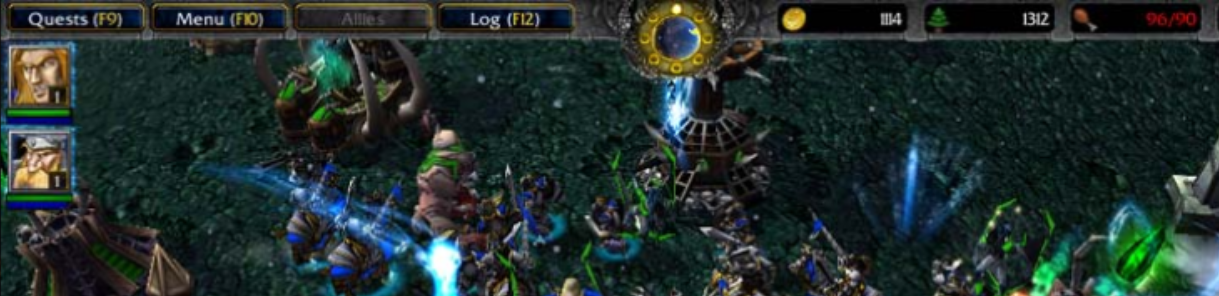
\includegraphics[width=0.9\textwidth]{images/ui/warcraft3.png}
    \caption{Pasek z informacjami oraz ikony dla dostępnych postaci w grze Warcraft 3}\label{fig:Warcraft3}
\end{figure}

W naszej grze skupimy się jednak na tym, aby Interfejs Użytkownika zabierał jak najmniej miejsca. Dlatego też projekt zakłada, że poszczególne obiekty nie będą ze sobą połączone tłem, zminimalizować zakrytą przestrzeń.
Jako ważny element tej części UI zawarty zostanie kompas, wzorowany na tym z gry The Elder Scrolls V: Skyrim.

\begin{figure}[htbp]
    \centering
    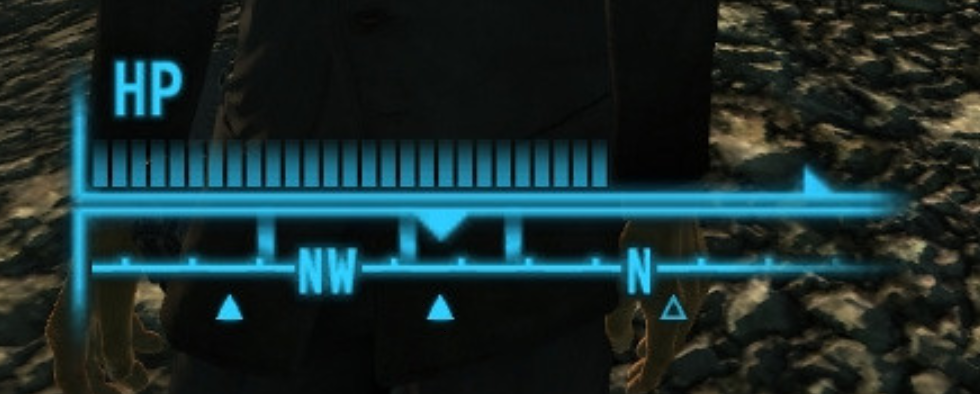
\includegraphics[width=0.9\textwidth]{images/ui/compassSkyrim.png}
    \caption{Kompas z gry Skyrim}\label{fig:Fallout}
\end{figure}


\begin{figure}[htbp]
    \centering
    
\includegraphics[width=0.9\textwidth]{images/ui/naszpasek.png}
    \caption{Projekt paska z najważniejszymi informacjami o stanie gry: aktualnym czasie, posiadanych surowcach i funduszach oraz o położeniu i otoczeniu gracza.
    }\label{fig:compass}
\end{figure}
 

 W trybie budowania informacje wcześniej przedstawione zostaną na ekranie. Dodatkowo   pokażą nam się dostępne do zbudowania budynki, a po wybraniu pojawią się przed nami. Po zatwierdzeniu budynek zostanie wybudowany.
	Inspiracją do przedstawienia dostępnych budowli jest rozwiązanie gry Orcs must die!

    \begin{figure}[h!tbp]
        \centering
        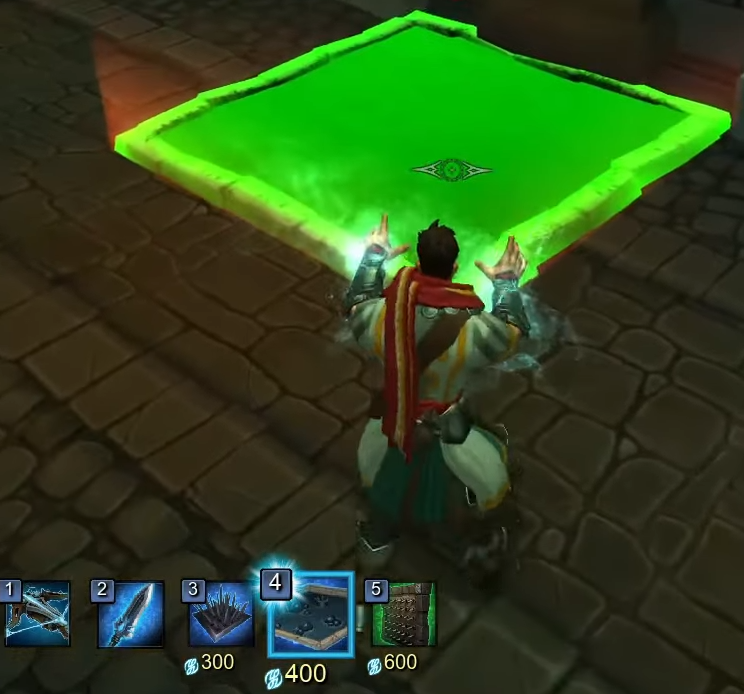
\includegraphics[width=0.9\textwidth]{images/ui/buoildingsOrcs.png}
        \caption{Wyświetlenie dostępnych pułapek w Orcs must die!}\label{fig:Orcs}
    \end{figure}


Bliźniaczo do trybu budowania, gdy rozpocznie się walka, podstawowe informacje zostają na ekranie, a dodatkowo gracz dostaje informacje o dostępnych rozkazach do wydania. Nasze rozwiązanie będzie podobne do pomysłu z gry Mount\&Blade.

\begin{figure}[h!tbp]
    \centering
    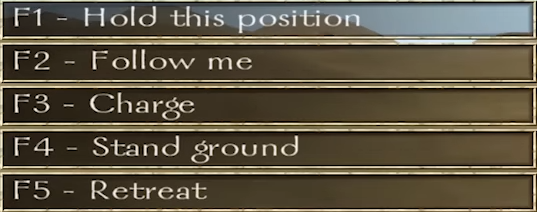
\includegraphics[width=0.9\textwidth]{images/ui/commandsMountBla.png}
    \caption{Wykaz dostępnych rozkazów z gry Mount\&Blade.}\label{fig:MountnBlade}
\end{figure}
